\documentclass[12pt, twocolumn]{article}

\usepackage[margin=0.75in]{geometry}
%\usepackage{tabularx}
\usepackage{amsmath}
\usepackage{amssymb}
%\usepackage{setspace}
\usepackage{graphicx}
\graphicspath{{./figure/}}
\usepackage{hyperref}
\usepackage{caption}
\usepackage{ulem}
%\usepackage[justification=centering]{caption}
%\usepackage{parskip} % replaces parindent and parskip
%\setlength{\parindent}{0pt}
%\setlength{\parskip}{1em}
%\pagestyle{empty}
%\usepackage{slashed}
%\usepackage{simplewick}
%\usepackage{datenumber}
%\usepackage{color}
\usepackage{multirow}
%\usepackage{feynmp} % Feynman Diagrams
%\DeclareGraphicsRule{*}{mps}{*}{} % Feynman Diagrams
%\usepackage[usenames,dvipsnames]{xcolor}
%\usepackage[utf8]{inputenc} % for accents in the names of citation
\usepackage{pdfpages}

\numberwithin{equation}{section}

\begin{document}
\sloppy % to relax the rules for inter word spacing making the word don't overflow
\setcounter{page}{0}

\title{Multi-documentation Summarization of Science Articles}
\author{Justin To, Luka Liu, Milan Dean}
\date{
    W 266: Natural language Processing
    \\UC Berkeley School of Information
    \\~
    \\\today
}

\onecolumn

\maketitle
\begin{abstract}%\normalsize\parindent 0pt\parskip 5pt

    In today's world, with an abundance of information available, the skill of generating accurate and concise summaries from extensive texts is more crucial than ever before. This study primarily focuses on the task of abstractive multi-document summarization (MDS), which involves generating a summary based on multiple interrelated documents. To build an MDS model tailored to Multi-XScience, a dataset that the pre-trained models have not encountered before, we explored different strategies such as fine-tuning and model-stacking, using two state-of-the-art pre-trained large language models (LLMs), namely Centrum and LED. In evaluating the generated summaries, we employed both quantitative ROUGE-based scoring and qualitative analysis of the model outputs to gain insights into how the models adapted to specific elements of the task and dataset. Our objective is to contribute to research on adapting pre-trained models to new and domain-specific MDS tasks and datasets using different approaches, such as fine-tuning and model stacking, and identify elements that may affect the success of such approaches.

\end{abstract}
\thispagestyle{empty}

\newpage
\twocolumn

\section{Introduction}

MDS is the task of summarizing multiple texts into a concise and informative summary. Compared to single document summarization, it is challenging to keep the summary coherent and comprehensive, given the documents are longer\footnote{For instance, the widely used CNN/Daily Mail dataset has an average input length of around 780 tokens.  In contrast, around 30\% of the inputs in the Multi-XScience dataset has over 1024 tokens, while the longest sample has over 6300 tokens.} and of a more complex structure\footnote{In MDS, the source articles are written by multiple authors with varying writing styles and article structures.}. Despite the challenges, MDS has wider application potential as real-world tasks often involve collating and summarizing information from multiple sources.  An important question therefore is, given the advances in NLP and the availability of pre-trained LLMs, how should we build a customized abstractive MDS model if we are given a domain-specific dataset previously unseen by the models?  

In this paper, we employ the Multi-XScience dataset, a relatively recent dataset that has not been widely used for pre-training/fine-tuning LLMs, to simulate the situation where we are given an MDS task for a broad domain, e.g.~academic writing from the sciences.  The defining characteristics of the dataset, namely (a) the significant portion of samples with long inputs (up to $\sim$6300 tokens) and (b) that different articles within each sample are related yet not covering the exact same event\footnote{Further discussed in Section~\ref{ssec:dataset}}, led us to pick two models for experimentation.  The first is the Longformer Encoder Decoder (LED) model, which was proposed by Beltagy et al.~\cite{beltagy2020longformer} and introduced the concept of local vs global attention so that attention-based transformers can still effectively handle the computation of long inputs.   The second is the Centrum model, proposed by Puduppully and Steedman~\cite{puduppully2022multidocument}, for its capability of handling long inputs and inclusion of a centroid-based approach for dealing with multiple source documents. 

Leveraging on the available pre-trained checkpoints, we first tested the off-the-shelf LED and Centrum using the Multi-XScience dataset and then proceeded to fine-tune them for improved performance.  Then, we explored the use of a two-step setup whereby individual source articles of each sample are first shortened through summarization, and then combined again for MDS processing.  For evaluation, we employed the common ROUGE score metric, showing the improved performance from fine-tuning (ROUGE-2 from 5.2 to 6.9; ROUGE-L from 14.6 to 17.8, which are close to state-of-the-art (SOTA)).  Further analyses were conducted on the variation of performance across inputs of different lengths, and the amount of ``copying'' from the main article.  Lastly, a qualitative analysis was done on 25 samples for each model tested, and the fine-tuned and two-step models were found to demonstrate capabilities in extracting information from and contrasting different sources, while adapting its writing style to one suited for the dataset.

\section{Related Works}
\label{sec:relatedworks}

In recent years, there has been significant research in the field of MDS, with a particular focus on the use of transformer-based models for abstractive models and through approaches such as sparse attention mechanisms, hierarchical sentence representations, and document-level clustering. Much progress has also been made in providing datasets for MDS training and evaluation.

On model development, the LED model proposed by Beltagy et al.~\cite{beltagy2020longformer} addresses the issue of processing long documents by introducing a sparse attention mechanism that allows the model to scale to documents of up to 16384 tokens. This approach has outperformed previous models, including advanced ones such as PEGASUS, on long-document tasks such as summarization.

Branching off to models more specialized in MDS, PRIMERA, proposed by Xiao et al.~cite{xiao2022primera}, is a pre-training method for transformer-based models that leverages hierarchical sentence representations to improve performance on MDS tasks. The approach involves constructing a sentence-level pyramid structure and applying a masked language modeling objective to the pyramid, leading to improved results over BART, PEGASUS, and LED.

Advancing the research on MDS further, Puduppully and Steedman~\cite{puduppully2022multidocument} proposed a centroid-based pre-training method for MDS that leverages document-level clustering to capture document-level semantics. This approach showed improved performance on summarization tasks over previous models including PRIMERA, particularly for MDS datasets with a large number of documents.

On the dataset front, a commonly used dataset in the MDS domain is perhaps the Multi-news dataset, which was introduced by Fabbri et al.~\cite{fabbri-etal-2019-multi} and contains news articles from multiple sources.  Other MDS datasets include Wikisum, which was generated by Liu et al.~\cite{liu2018generating} from Wikipedia articles, WCEP compiled by Ghalandari at el.~\cite{ghalandari2020largescale} based on news summaries from the Wikipedia Current Events Portal, and the Multi-XScience dataset by Lu et al.~\cite{lu-etal-2020-multi-xscience} used in this study.  

\section{Methods}
\label{sec:methods}

\subsection{Dataset}
\label{ssec:dataset}

We used the Multi-XScience MDS dataset~\cite{lu-etal-2020-multi-xscience} in this study, which is a collection of scientific articles from scientific fields, including computer science, physics, and biology.  Some key parameters of the dataset are set out as follows, while Appendix~\ref{app:eda} summarizes other findings and visualizations from our EDA, as well as the data preprocessing steps adopted for the experiments.  

\begin{table}
    \small
    \begin{tabular}{|l|c|c|c|}
    \hline
        ~ & Training & Validation & Test  
        \\ \hline
        Sample size & 30369 & 5066 & 5093 
	\\ \hline
        \shortstack{Input\\Token Length}
	    & \shortstack{899 \\ 565 \\ 82-4694}
	    & \shortstack{898 \\ 567 \\ 79-4183}
	    & \shortstack{886 \\ 547 \\ 131-6348}
	\\ \hline
        \shortstack{Samples with\\inputs $>1024$\\tokens} & 31.21\% & 30.71\% & 30.87\% 
        \\ \hline
        \shortstack{Label\\Token Length}
	    & \shortstack{142 \\ 58 \\ 24-735}
	    & \shortstack{141 \\ 58 \\ 25-324}
	    & \shortstack{142 \\ 58 \\ 26-418}
	\\ \hline
        \shortstack{Articles per\\sample}
	    & \shortstack{4.43 \\ 2.62 \\ 2-21}
	    & \shortstack{4.43 \\ 2.63 \\ 2-20}
	    & \shortstack{4.39 \\ 2.55 \\ 2-19}
	 \\ \hline
    \end{tabular}
    \caption{Dataset description. The cells with three columns refer to mean/standard deviation/range}
    %\footnote{Based on the tokenizer of LED which is based on that of BART and shares the vocabulary with Centrum.}
\end{table}

%\begin{table*}[!ht]
%    \centering
%    \small
%    \begin{tabular}{|l|c|c|c|}
%    \hline
%        ~ & Training & Validation & Test
%        \\ \hline
%        Sample size & 30369 & 5066 & 5093 
%	\\ \hline
%        Input Token Length
%	    & \shortstack{899 \\ (s.d.: 565) \\ (range: 82 - 4694)}
%	    & \shortstack{898 \\ (s.d.: 567) \\ (range: 79 - 4183)}
%	    & \shortstack{886 \\ (s.d.: 547) \\ (range: 131 - 6348)}
%	\\ \hline
%        Samples with inputs $>1024$ tokens & 31.21\% & 30.71\% & 30.87\% 
%        \\ \hline
%        Label Token Length 
%	    & \shortstack{142 \\ (s.d.: 58) \\ (range: 24 - 735)}
%	    & \shortstack{141 \\ (s.d.: 58) \\ (range: 25 - 324)}
%	    & \shortstack{142 \\ (s.d.: 58) \\ (range: 26 - 418)}
%	\\ \hline
%        Articles per sample 
%	    & \shortstack{4.43 \\ (s.d.: 2.62) \\ (range: 2 - 21)}
%	    & \shortstack{4.43 \\ (s.d.: 2.63) \\ (range: 2 - 20)}
%	    & \shortstack{4.39 \\ (s.d.: 2.55) \\ (range: 2 - 19)}
%	 \\ \hline
%    \end{tabular}
%    \caption{Dataset description}
%    %\footnote{Based on the tokenizer of LED which is based on that of BART and shares the vocabulary with Centrum.}
%\end{table*}

The dataset is chosen for two reasons.  First, Multi-XScience is among the few datasets previously unseen by MDS models during pre-training\footnote{LED’s pre-training data included Multi-News while Centrum’s pre-training included both Multi-News and WikiSum.}. Picking datasets already seen by the models could pose difficulties in evaluation, not to mention that it would go against the overall goal to explore MDS model-building strategies for unseen data. 

The second reason is that Multi-XScience is a more challenging task that is more comparable to real-world data collation and summarization.   Many of the datasets (e.g.~Multi-news, WCEP) are news-based, with the articles within a sample covering the same news event and key elements to be included in the summary appearing in multiple sources.  The Multi-XScience dataset however, expects the model to write the related works section of a journal paper based on (a) the abstract of that paper which serves to provide context; and (b) the abstracts of the other journal articles that the main paper referenced.  While these additional abstracts are usually\footnote{Some exceptions exist, e.g.~sample 845 (refer to Appendix~\ref{app:samples} for sample review for sample review)) of the test set includes an irrelevant article on the design attributes of luggage carriers when the main article is on a MDS over online product reviews.  See ~Appendix~\ref{app:qualitative} for details.} closely related, they often concern different aspects of an issue, and the model needs to be able to compare and contrast the similarities and differences\footnote{In contrast, the commonly used Multi-news dataset has, in each sample, multiple news reports surrounding a single event, and the overall theme to be covered in the summary is generally present in every source article.}.  This difficulty of the dataset also shows up empirically\footnote{For instance, the zero- and few-short evaluation of BART, PEGASUS, LED and PRIMERA yielded a ROUGE-2 score of only 1.9 to 4.6 and a ROUGE-L score of 9.9 to 15.7 for Multi-XScience, while the score ranges for Multi-news is 3.7 to 13.6 for ROUGE-2 and 10.4 to 20.8 for ROUGE-L.  A similar gap remains even after fine-tuning of the models.} in~\cite{xiao2022primera}.

As can be seen from the table above, the input length of the Multi X-Science dataset shows great variability, with some inputs so short that they can fit in more traditional summarization models, while others exceed even 4096, which is the max input length for Centrum.  The same variability can also be observed in terms of the number of articles per sample (see Figure~\ref{fig:token-length} below), with the two distributions showing a close-to-linear pattern.  This provides an opportunity for us to use the Multi X-Science dataset to explore possible differences in model performance between short and long samples. 

\begin{figure}
    \captionsetup{width=\columnwidth}
    %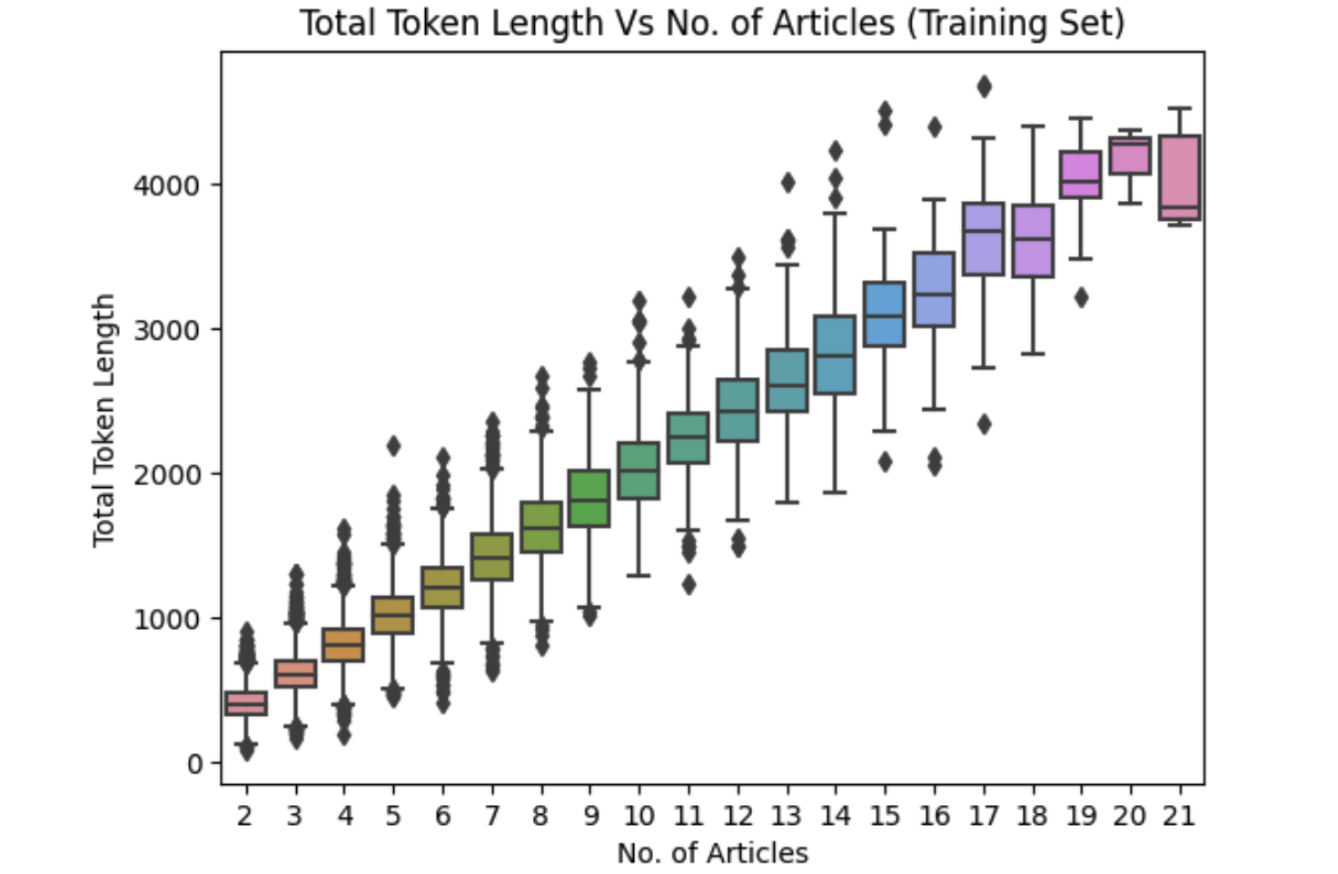
\includegraphics[width=\textwidth]{token_length.png}
    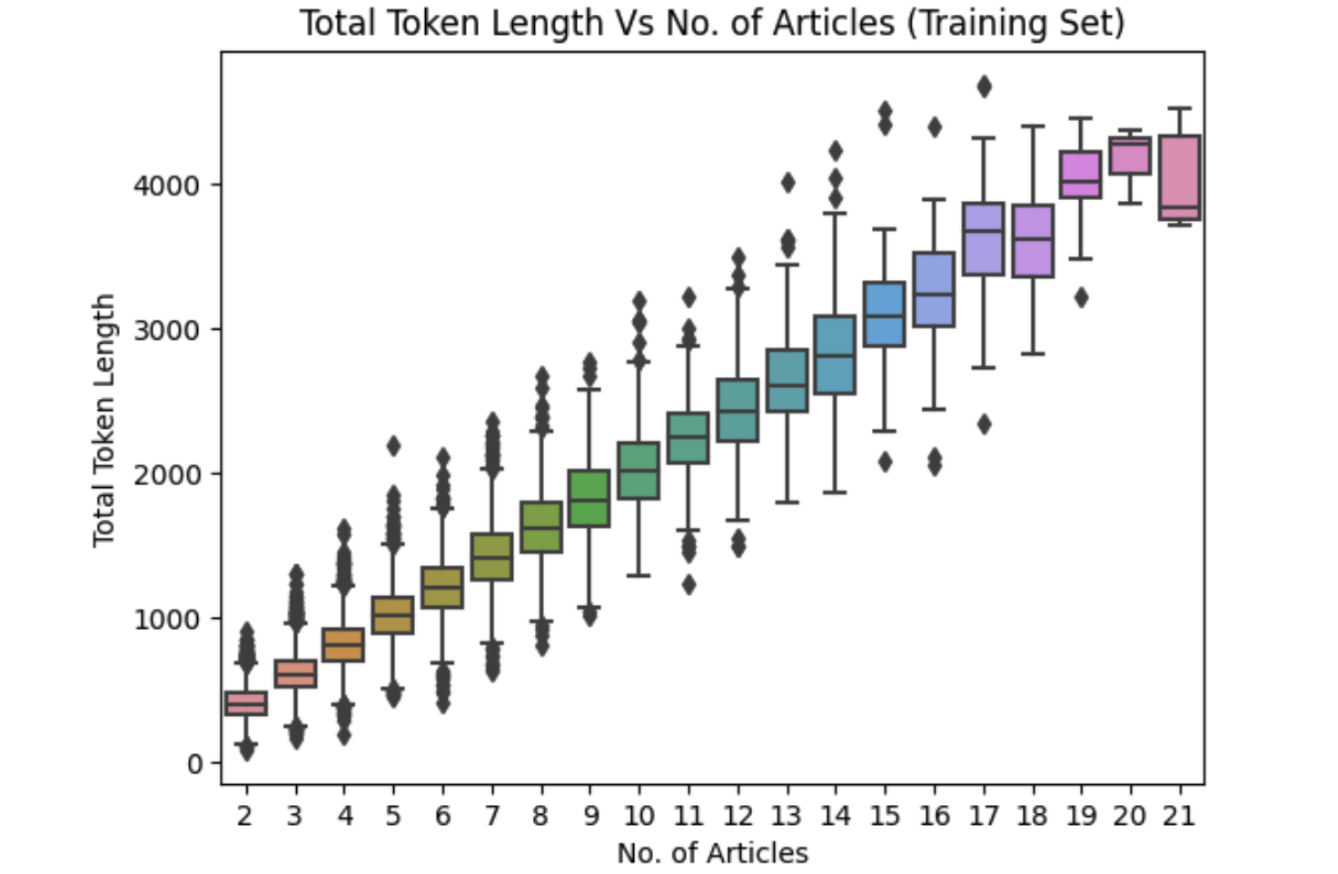
\includegraphics[width=\columnwidth]{token_length.png}
    \caption{Total token length as a function of the number of articles in the training data set. The relationship between token length and the number of articles is linear.}
    \label{fig:token-length}
\end{figure}

\subsection{Models}
\label{ssec:models}

Due to resource constraints, we focused on two pre-trained LLMs, namely LED and Centrum for our experiments.  Of the three recent and well-performing models we reviewed, we did not pick PRIMERA for two reasons - (a) Centrum is, based on literature review, the best-performing model while LED is a common starting point for both PRIMERA and Centrum, meaning it could be treated as a more advanced baseline; and (b) the authors of PRIMERA already provided performance results of PRIMERA on the Multi-XScience test set. 

We adopted two different baselines for performance comparison.  The first one, dubbed the ``baseline model'' is simply a lead-based model, whereby the first 3 sentences are chosen as the summary and is a common primary strategy implemented in various papers (e.g.~\cite{lu-etal-2020-multi-xscience}, \cite{see2017point} and \cite{zhang2020pegasus}).  This also provides a useful baseline for comparing the degree of ``copying'' (see Section~\ref{ssec:eval-metrics}) from the main article which is an undesirable trait for the chosen dataset.  The second baseline is the publicly available checkpoint for LED, which serves as the base architecture for recent MDS LLMs.  

On top of the 2 baseline models, we ran experiments on the performance of the following models, with details on their fine-tuning and inference settings provided in Appendix~\ref{app:model}:

\begin{enumerate}
    \item an alternative checkpoint of LED fine-tuned on the arXiv dataset
    \item publicly available checkpoint of Centrum;
    \item a version of the baseline LED\footnote{In theory, it would be better to fine-tune the alternative LED checkpoint which (a) is a larger version of LED with double the parameters; and (b) has been fine-tuned on text from the scientific fields.  However, the GPU we had was unable to train the larger model while maintaining the max input token length at a reasonable level.} that we fine-tuned on the Multi-XScience training set; 
    \item a similarly fine-tuned version of Centrum; and
    \item a two-step model stacking the fine-tuned LED and Centrum.
\end{enumerate}

Of these experiments, models (c) and (d) stem from our plan to test out the performance of fine-tuning strategies for MDS.  During the process, we noticed that despite the larger input length of Centrum (4096 tokens), there are still cases where the inputs have to be truncated and information omitted.  We therefore explored under model (e) a two-step model stacking process whereby the source articles are first condensed by our fine-tuned LED individually followed by an MDS process by (a) the fine-tuned LED or (b) the fine-tuned Centrum.  The idea is to investigate if Centrum performs better when presented with more concise sources and without token truncation, see Figure~\ref{fig:two-steps}. Refer to Appendix~\ref{app:model} for more details on the two step model.

\begin{figure}
    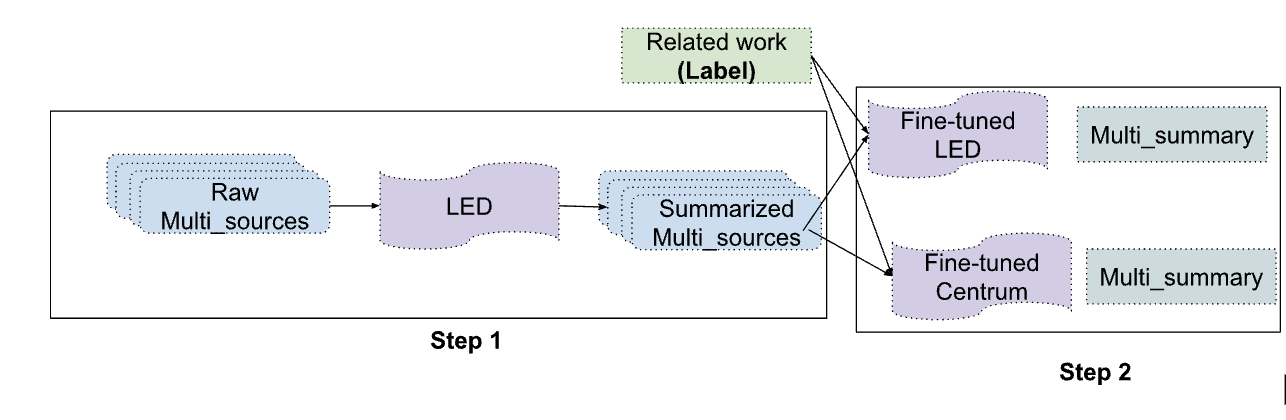
\includegraphics[width=\columnwidth]{two_steps.png}
    \caption{Two-steps model design}
    \label{fig:two-steps}
\end{figure}

\subsection{Evaluation metrics}
\label{ssec:eval-metrics}

As in the standard practice for summarization, the primary metric we use is the ROUGE score.  Among the different versions of ROUGE, we chose ROUGE-2 and ROUGE-L, with a particular focus on the latter given the prevalence of compound nouns in academic writings\footnote{This is an empirical observation from viewing samples in the dataset, and is quite intuitive considering academic terms are often ones glued together from multiple words (e.g.~the theme of ``Synchronous Optical Network Ring Assignment Problem'' in sample 4820 of the test set, and ``fixed-size ordinally forgetting encoding'' in sample 3157).}, for gauging model performance.  Compared to ROUGE-2, ROUGE-L is better suited for this task.  In calculating these metrics, precision, recall, and f-measure are all considered\footnote{We also look only at the mean score but not the lower and upper ranges due to the limited scope of our study, though we recognize that looking at the variation in performance across samples is in itself a valid future investigation direction.}, and scores were computed for the overall test dataset, as well as the subsets of short, medium, and long token length samples\footnote{We divided the 5093 test samples into three groups.  ``Short'' samples consisted of 1273 samples with less than 486 tokens (lower quartile) for the inputs; ``medium'' with 2546 samples with input lengths between 486 and 735 (upper quartile) tokens; and the remaining 1274 samples with input lengths greater than 1150 tokens are grouped into the ``long'' samples.}.  

Unlike other MDS datasets where the key information is expected to be found in most, if not all, of the source articles, the Multi X-Science dataset has a different structure whereby the main article (i.e. first source) is expected to provide general context while the other sources will each provide a related, yet different angle of the topic.  It is desirable for models to extract information not just from the main article, and we therefore measured the degree of ``copying'' from the main article by repurposing standard ROUGE calculations\footnote{Implemented using the standard rouge function by replacing the target reference that the function takes in with the main article of the sample.}.

Finally, we supplemented our evaluation with a qualitative analysis whereby 25 random samples were selected and we reviewed the summaries written by the baseline LED and the 5 models experimented, judging them based on fluency, ability to extract information from multiple sources, and contrast information from the main article and other sources, as well as factual accuracy.

\section{Results and Discussion}
\label{sec:results}

\subsection{Overall performance}
\label{ssec:results-overall}

In the following table, we report the ROUGE-2 (R-2) and ROUGE-L (R-L) scores of the 2 baselines plus 5 models we tested, with precision (P), recall (R), and f-measure (F) scores presented.  Scores for overall, short, medium, and long samples are also presented.

As shown in the tables above, the fine-tuned models (LED and Centrum) provided a markedly improved performance over the baselines and off-the-shelf models.  In fact, even though the models were only fine-tuned for up to 2 epochs\footnote{Training details and considerations are at Appendix~\ref{app:model}.}, our figures quickly approached the SOTA figures reported in~\cite{xiao2022primera} (i.e.~ROUGE-2 of 6.8; ROUGE-L of 18.2) demonstrating the viability of LED and Centrum to be adopted for previously unseen MDS data.  When considering the breakdowns, the improvement for longer samples was much more visible, indicating the MDS-specific model architectures are perhaps more suitable for tasks with longer input lengths.  

This result is consistent with what our qualitative analysis (Appendix~\ref{app:qualitative}).  For example, in sample 485, the Centrum model was able to extract the key ideas of 3 relevant studies and contrast them with the main article, forming a coherent summary, while the baseline and off-the-shelf models were overwhelmed by the large number of articles (9 in total) and choose only to copy one of the articles in full.  This is very different from shorter samples, e.g.~sample 4160 with only 3 articles, where the off-the-shelf models were still able to prepare a summary covering elements, albeit in a more extractive manner without efforts to change the tone or merge the extracted parts together.

For the two-step model, the ROUGE scores do not show any advantage of the approach over simple fine-tuned models.  However, as we observe from the qualitative analysis (e.g.~samples 831 and 5068), there is a strong tendency for the two-step model to highlight differences and similarities between the main and other articles.  However, the downside is that the two-step model made quite a number of factual fallacies in the process\footnote{One possible reason is that we need better tuning on the amount and manner of information fed into the 2nd step model, but resouce limitations were a main obstacle considering the generation of the first step answers alone took over 14 hours.}.

\begin{table}
    \centering
    \footnotesize
    \begin{tabular}{|p{1.5cm}|c|c|c|c|c|}
    \hline
        Model & R-2 & Overall & Short & Medium & Long \\ \hline
        \multirow{3}{1.5cm}{Baseline (Lead)} & P & 4.50 & 4.78 & 4.68 & 3.87 \\ \cline{2-6}
        & R & 8.13 & 6.12 & 7.87 & 10.7 \\ \cline{2-6}
        & F & 5.40 & \textit{5.02} & 5.56 & 5.48 \\ \hline
        \multirow{3}{1.5cm}{Baseline (LED)} & P & 4.52 & 4.12 & 4.75 & 4.47 \\ \cline{2-6}
        ~ & R & 6.99 & 8.17 & 7.07 & 5.63 \\ \cline{2-6}
        ~ & F & \textit{5.21} & 5.2 & 5.40 & \textit{4.83} \\ \hline
        \multirow{3}{1.5cm}{LED} & P & 5.25 & 5.32 & 5.30 & 5.09 \\ \cline{2-6}
        ~ & R & 6.31 & 6.97 & 6.34 & 5.57 \\ \cline{2-6}
        ~ & F & 5.39 & 5.58 & 5.44 & 5.11 \\ \hline
        \multirow{3}{1.5cm}{Centrum} & P & 4.14 & 4.02 & 4.23 & 4.09 \\ \cline{2-6}
        ~ & R & 8.12 & 9.48 & 8.14 & 6.70 \\ \cline{2-6}
        ~ & F & 5.24 & 5.36 & \textit{5.34} & 4.93 \\ \hline
        \multirow{3}{1.5cm}{Our LED} & P & 8.75 & 8.03 & 8.67 & 9.63 \\ \cline{2-6}
        ~ & R & 5.89 & 5.21 & 5.69 & 6.94 \\ \cline{2-6}
        ~ & F & 6.56 & 5.83 & 6.41 & 7.62 \\ \hline
        \multirow{3}{1.5cm}{Our Centrum} & P & 7.62 & 7.10 & 7.58 & 8.28 \\ \cline{2-6}
        ~ & R & 7.27 & 6.38 & 7.13 & 8.44 \\ \cline{2-6}
        ~ & F & \textbf{6.88} & \textbf{6.14} & \textbf{6.78} & \textbf{7.82} \\ \hline
        \multirow{3}{1.5cm}{2-Step (Centrum)} & P & 5.87 & 5.66 & 5.92 & 5.99 \\ \cline{2-6}
        ~ & R & 6.67 & 6.15 & 6.62 & 7.26 \\ \cline{2-6}
        ~ & F & 5.86 & 5.42 & 5.87 & 6.28 \\ \hline
    \end{tabular}
    \caption{Rouge-2 Scores for Models Tested (Best in \textbf{bold}; worst is \textit{italicized})}
    \label{tab:rouge-2}
\end{table}

\begin{table}
    \centering
    \footnotesize
    \begin{tabular}{|p{1.5cm}|c|c|c|c|c|}
    \hline
        Model & R-2 & Overall & Short & Medium & Long \\ \hline
        \multirow{3}{1.5cm}{Baseline (Lead)}
	& P & 12.4 & 14.9 & 12.7 & 9.17 \\ \cline{2-6}
        & R & 21.7 & 18.8 & 21.3 & 25.2 \\ \cline{2-6}
        & F & 14.6 & 15.5 & 15 & \textit{12.9} \\ \hline
        \multirow{3}{1.5cm}{Baseline (LED)} 
	& P & 12.9 & 11.6 & 13.3 & 13.5 \\ \cline{2-6}
        & R & 20.5 & 23.8 & 20.4 & 17.3 \\ \cline{2-6}
        & F & 14.9 & 14.8 & 15.1 & 14.6 \\ \hline
        \multirow{3}{1.5cm}{LED} 
	& P & 15.1 & 15.4 & 15.1 & 14.3 \\ \cline{2-6}
        & R & 18.6 & 20.3 & 18.7 & 16.7 \\ \cline{2-6}
        & F & 15.7 & 16.2 & 15.7 & 15.0 \\ \hline
        \multirow{3}{1.5cm}{Centrum} 
	& P & 11.3 & 10.8 & 11.4 & 11.7 \\ \cline{2-6}
        & R & 22.7 & 25.5 & 22.8 & 19.7 \\ \cline{2-6}
        & F & \textit{4.4} & \textit{14.4} & \textit{14.6} & 14.2 \\ \hline
        \multirow{3}{1.5cm}{Our LED} 
	& P & 23.6 & 24.2 & 23.5 & 23.2 \\ \cline{2-6}
        & R & 15.9 & 15.7 & 15.5 & 16.8 \\ \cline{2-6}
        & F & 17.7 & 17.6 & 17.4 & \textbf{18.4} \\ \hline
        \multirow{3}{1.5cm}{Our Centrum} 
	& P & 19.8 & 20.9 & 19.6 & 19.1 \\ \cline{2-6}
        & R & 18.9 & 18.4 & 18.7 & 19.7 \\ \cline{2-6}
        & F & \textbf{17.8} & \textbf{17.9} & \textbf{17.6} & 18.1 \\ \hline
        \multirow{3}{1.5cm}{2-Step (Centrum)} 
	& P & 17.0 & 18.0 & 17.0 & 15.9 \\ \cline{2-6}
        & R & 19.6 & 19.7 & 19.5 & 19.6 \\ \cline{2-6}
        & F & 17.0 & 17.4 & 17.0 & 16.7 \\ \hline
    \end{tabular}
    \caption{Rouge-L Scores for Models Tested (Best in \textbf{bold}; worst is \textit{italicized})}
    \label{tab:rouge-l}
\end{table}

\subsection{Degree of Copying}
\label{ssec:results-copy}

To assess the degree of copying from the main article, we calculated a re-purposed ROUGE-L score. As shown in the table below, the fine-tuned and two-step models exhibited a significantly lower degree of ``copying'', which is supported by the qualitative analysis showing that these models were able to extract information from multiple articles. In contrast, the baseline LED model showed the highest degree of ``copying'', often copying substantial portions of the main article to the point that the number of copied sentences exceeded even that of the lead-based baseline.

Although the ROUGE scores did not reveal any significant ``copying'' for the off-the-shelf LED and Centrum models, it is noteworthy that these models occasionally copied from a single reference article rather than the main article (e.g.~see the output of the base Centrum for sample 4371). This indicates that there is still room for improving the ``copying'' metric, such as by taking the minimum of the ROUGE-L scores compared to each input article (rather than just the main article) to discourage ``copying'' from a single source.

\begin{table}
    \centering
    \footnotesize
    \begin{tabular}{|p{1.5cm}|c|c|c|c|c|}
    \hline
        Model & R-2 & Overall & Short & Medium & Long \\ \hline
        \multirow{3}{1.5cm}{Baseline (Lead)} 
	& P & 39.7 & 56.6 & 39.7 & 22.7 \\ \cline{2-6}
        & R & 40.7 & 41.1 & 39.0 & 43.9 \\ \cline{2-6}
        & F & 36.8 & 44.9 & 36.8 & 28.5 \\ \hline
        \multirow{3}{1.5cm}{Baseline (LED)} 
	& P & 76.9 & 83.1 & 86.9 & 50.7 \\ \cline{2-6}
        & R & 75.5 & 92.8 & 81.5 & 46.3 \\ \cline{2-6}
        & \textit{F} & \textit{74.2} & \textit{85.6} & \textit{81.9} & \textit{47.2} \\ \hline
        \multirow{3}{1.5cm}{LED} 
	& P & 45.3 & 58.8 & 43.9 & 34.7 \\ \cline{2-6}
        & R & 33.6 & 44.3 & 31.5 & 27.0 \\ \cline{2-6}
        & F & 37.4 & 48.9 & 35.6 & 29.5 \\ \hline
        \multirow{3}{1.5cm}{Centrum} 
	& P & 48.2 & 56.5 & 48.6 & 39.2 \\ \cline{2-6}
        & R & 57.5 & 73.7 & 55.7 & 45.1 \\ \cline{2-6}
        & F & 51.2 & 62.4 & 50.8 & 41.0 \\ \hline
        \multirow{3}{1.5cm}{Our LED} 
	& P & 33.6 & 35.5 & 34.7 & 29.5 \\ \cline{2-6}
        & R & 13.5 & 13.0 & 13.2 & 14.7 \\ \cline{2-6}
        & \textbf{F} & \textbf{18.3} & \textbf{18.0} & \textbf{18.2} & 18.7 \\ \hline
        \multirow{3}{1.5cm}{Our Centrum} 
	& P & 29.4 & 32.9 & 29.4 & 26.1 \\ \cline{2-6}
        & R & 17.3 & 16.4 & 16.9 & 19.0 \\ \cline{2-6}
        & F & 20.5 & 20.7 & 20.1 & 20.9 \\ \hline
        \multirow{3}{1.5cm}{2-Step (Centrum)} 
	& P & 24.7 & 27.9 & 25.0 & 21.0 \\ \cline{2-6}
        & R & 17.2 & 17.1 & 16.8 & 18.0 \\ \cline{2-6}
        & F & 19.1 & 20.1 & 18.9 & \textbf{18.6} \\ \hline
    \end{tabular}
    \caption{Rouge-L Scores for Measuring ``Copying'' (Best in \textbf{bold}; worst is \textit{italicized})}
    \label{tab:rouge-l-copy}
\end{table}

\subsection{Other observations}
\label{ssec:results-other}

The qualitative analysis also allowed us to make the following observations on the models, including:

\begin{enumerate}
    \item The fine-tuned and two-step models showed clear signs of learning common writing styles (using phrases such as ``there is a large body of work...'') which is desirable in real world applications;
    \item For samples containing irrelevant articles, the fine-tuned models were able to safely navigate away from them (e.g.~sample 845)
    \item Despite having been fine-tuned on journal articles, the models showed greatest difficulties when presented with highly technical papers that use common words in uncommon meanings (e.g.~in mathematics in sample 4858).  This shows the potential to enhance performance by adding another fine-tuning step on domain-specific texts.  Alternatively, the two-step model has continued to perform well in such cases which shows the potential of such an approach.
\end{enumerate}

\section{Conclusion}
\label{sec:conclusion}

In conclusion, we demonstrated the viability of building custom-based MDS models through fine-tuning which is able to quickly approach SOTA scores even with simple and limited tuning.  Through breakdown and qualitative analyses of the results, we highlighted the importance of considering the token length of input texts when selecting a text summarization model. Our results suggest that the fine-tuned LED and Centrum models are much more adept at MDS for longer texts, while the two-step model shows potential especially for highly technical texts despite needing more tuning. Future work could focus on further optimizing the tuning techniques (e.g.~fine-tuning with domain-specific texts first before the MDS data), improving on the two-step approach, as well as looking at the performance stability of the models across data samples.

\newpage
\textbf{\Huge Appendix}
\appendix

\section{EDA and Data Preprocessing}
\label{app:eda}

\subsection{Introduction}
\label{app:eda-intro}

This appendix provides further findings from the EDA on the Multi-XScience dataset, as well as the data preprocessing procedures undertaken in the experiments. In particular, the distribution in the length of inputs and labels respectively guided us in determining (a) the maximum number of tokens fed into the models; and (b) the maximum output of length of generated summaries.

\subsection{Distribution of Input and Output Lengths}

To determine the input length, we looked at the average length of the samples (i.e.~each with multiple articles) in the Multi-XScience dataset.  Based on the parameters set out in Table 1 of the paper, and taking into account model limitations\footnote{LED can take in at most 16384 tokens and Centrum can take in 4096 tokens.} and GPU capabilities, we set the input numbers of tokens as 4096 in the fine-tuning process.  As for the baseline and off-the-shelf models which do not require fine-tuning, we experimented on other input token lengths including 512, 1024 and 16384. 

To determine the max output length\footnote{LED and Centrum both do not come with options to set minimum output lengths.  One can force such a parameter into the generation function, but initial experimentations showed minimal impact on the output.}, we looked at the distribution of the token length of the standard summaries (label) that came with the dataset.  A sample distribution for the training dataset, which closely resembles the distributions for the validation and test datasets, is provided below.

\begin{figure}
    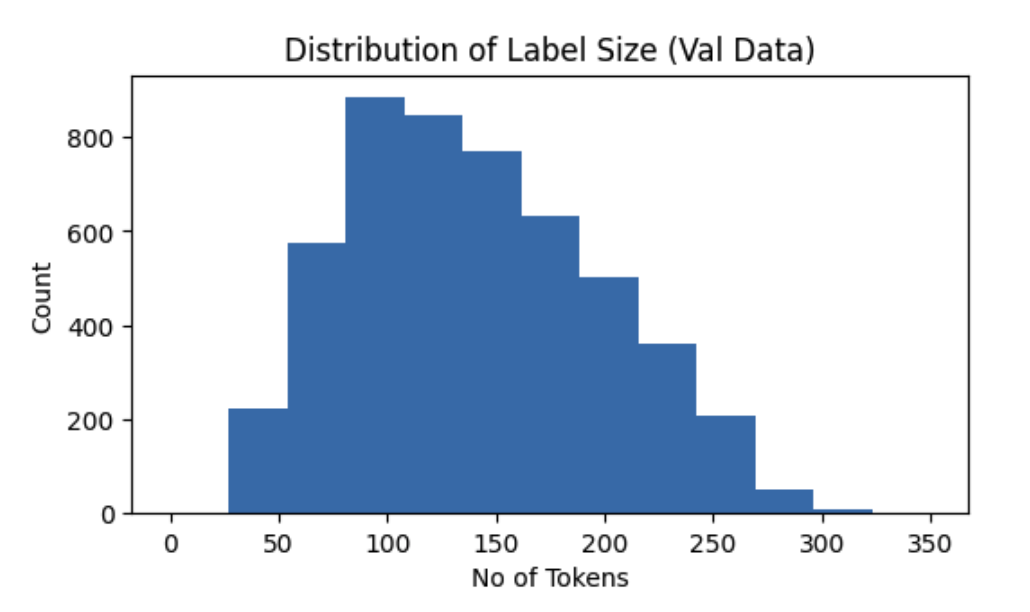
\includegraphics[width=\columnwidth]{label_dist.png}
    \caption{Distribution of the number of tokens in the label of training data. The number of tokens is right-skewed and centered around 100.}
    \label{fig:label-dist}
\end{figure}

Considering the desired level of detail in the summary and the distribution of standard summaries (label) tokens, we decided to set 256 as the maximum number of tokens\footnote{During a number oe early stage experiments with LED, the maximum was set at 200 instead.} at inference time.

\subsection{Data Preprocessing}

Multi-XScience includes a main abstract, which is from the main article; a standard summary of the related works with a separation of ``@cite'', which is the summary of multi-source documentations, label datasets; and reference abstracts, which are the multiple abstracts from a different source of works. We processed the dataset by defining the separator of documents as ``\texttt{|||||}'', a document separator, then concatenating reference abstracts using the document separator to replace citation references. 

\begin{figure*}
    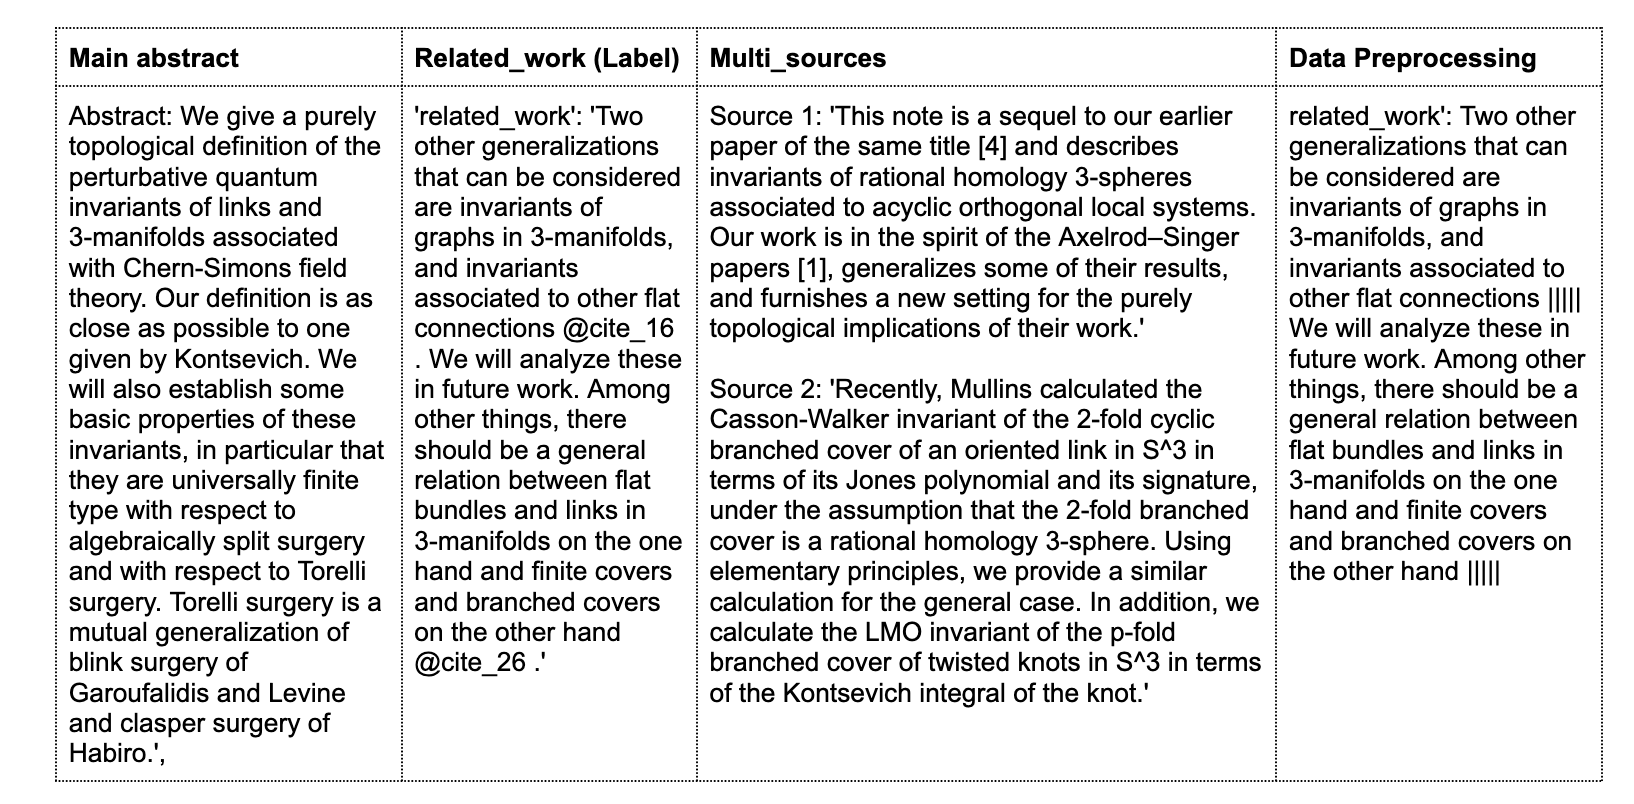
\includegraphics[width=\textwidth]{X_science_example.png}
    \caption{Multi-XScience data sample}
\end{figure*}

\section{Model}
\label{app:model}

\subsection{Baseline Model}
\label{app:model-baseline}

Copying the first 3 sentences from each reference abstract was used as our first baseline. It is a simple and easy-to-implement approach that provides a starting point for summarizing multiple documents. It assumes that the first few sentences of a document contain important information that should be included in the summary.

This approach can serve as a useful baseline for several reasons:

\begin{enumerate}
    \item It is easy to implement and does not require a lot of computational resources. This makes it a good starting point for developing more advanced summarization models.
    \item It is straightforward to understand and explain. This makes it a good choice for initial experiments and evaluations.
    \item It can provide a quick estimate of the performance of a summarization system. By comparing the summaries generated by this approach to human-written summaries or other machine-generated summaries, it is possible to get a rough idea of how well the system is performing.
\end{enumerate}

\subsection{Baseline Base LED (1K and 16K) Model}
\label{app:model-base-led}

The base LED model has (``allenai/led-base-16384''), with max input token length of 16384 \& $\sim$200M parameters and consists of 12 transformer encoder layers and 2 transformer decoder layers. This model is designed to be computationally efficient and suitable for low-resource environments. The baseline LED was generated based on a pre-trained LED model by Beltagy, L (2020)~\cite{beltagy2020longformer} on Multi-XScience test datasets with input tokens varying from 1k and 6k. 

\subsection{Off-the-shelf LED (1K and 16K) Model}
\label{app:model-large-led}

The off-the-shelf LED is referred to the ``large LED'' during our experiments to indicate that it has more parameters and is larger than the ``baseline'' LED model. The model has (``allenai/led-large-16384-arxiv''), with max input token length of 16384 \& $\sim$512M parameters, and consists of 24 transformer encoder layers and 4 transformer decoder layers. This model has been pre-trained for general summarization tasks. The baseline LED was generated based on a pre-trained large LED and evaluated on Multi-XScience test datasets.

\subsection{Off-the-shelf Centrum Model}
\label{app:model-centrum}

The ``ratishsp/Centrum'' model with max input token length of 4096 \& $\sim$192M parameters and consists of 12 transformer encoder layers and 12 transformer decoder layers. It is smaller than some of the larger transformer models, such as T5 and GPT-3, but larger than some of the smaller transformer models, such as the BART base. The publicly available Centrum checkpoint was built upon the LED model architecture using the 4096 token version.This means Centrum is not able to take in 16384 tokens.

\subsection{Fine-tuned LED Model}
\label{app:model-ft-led}

Fine-tuning the ``LED-large-16384-arxiv'' model to the Multi-XScience train (size 30369) and validation (size 5066) datasets specifically for the related work summarization. We used 4096 max number of tokens when feeding the training and validation sets during fine-tuning, and used 200 as the max output tokens with a batch size of 2 (due to limited GPU resources) at inference time. The model is then used as a cross-entropy loss function for 2 epochs with 40 checkpoints generated for every 5% of the training set fed into it, and evaluated on test datasets(size 5093) with ROUGE metrics. After looking into the performance of the checkpoints, we picked the 30th checkpoint (i.e.~trained for 1.5 epochs) as the final model.

\subsection{Fine-tuned Centrum Model}
\label{app:model-ft-centrum}

Fine-tuning the ``ratishsp/Centrum'' model to the X-science train and validation datasets specifically for the related works summarization.  We used 4096 max number of tokens when feeding the training and validation sets during fine-tuning, and used 256 as the max output tokens with a batch size of 1 (due to limited GPU resources) at inference time. The model is then used as a cross-entropy loss function for 2 epochs, and evaluated on test datasets (size 5093) with ROUGE metrics.

\subsection{Two-step LED/Centrum Model}
\label{app:model-two-step-led}

In the first step, the LED model is used to generate a summary of each related source document. By summarizing each source document, the model can condense the information and reduce redundancy, making it easier to process and analyze. For the first step, none of the individual source articles in the Multi-XScience dataset contain more than 4096 tokens, so there is no issue of the first step model (i.e.~the fine-tuned LED) receiving truncated inputs.

In the second step, generate the summary based on the fine-tuned LED model to refine the summaries generated in the first step. In this way, we were hoping that the second model can learn to generate even more accurate and relevant summaries.  Two different models were tested in the second step, namely our fine-tuned LED and the fine-tuned Centrum.  Only the results of the latter, which proved superior, were reported in the paper.

\subsection{Two-step Model results}
\label{app:model-two-step-model-results}

However, from our evaluation and observation of this approach, the performance of the two-step model does not exceed the fine-tuned LED/Centrum model. One potential issue is that the large amount of information contained in the source documents may make it difficult for the model to generate concise and informative summaries. Ultimately, the performance is heavily dependent on the performance of step 1. 

Overall, our results demonstrate the importance of utilizing advanced techniques like fine-tuning to unlock the full potential of language models in real-world applications.

\section{Qualitative Analysis}
\label{app:qualitative}

We also investigated how the model performed when summarizing short, medium, and long documents. The study aimed to evaluate the quality of the generated summaries and identify any trends or patterns in the model's performance based on the length of the source documents. A total of 25 randomly drawn samples (from the 5093 samples in the X-Science test dataset) are analyzed.  These 25 samples include:

\begin{itemize}
    \item 10 short samples, i.e.~with total token lengths below the lower quartile
    \item 10 medium samples, i.e.~with total token lengths between the lower and upper quartiles
    \item 5 long samples, i.e.~with token lengths above the upper quartile
\end{itemize}

Our analysis of the review (refer to the Analysis Appendix for more detailed review) results showed that the fine-tuned LED and Centrum learned the structure for multi-documents summary for X-science dataset, with particularly good results for longer documents (ref.~Sample 485) while for shorter samples the advantage over the baseline and off-the-shelf models appear to be less as those models are able to extract information from multiple sources to some degree, albeit with limited ability to merge them into a single coherent summary (ref.~Sample 4160). 

Additionally, we observed that LED and Centrum seem to have difficulties in digesting some of the more technical topics, where the use of common language for unusual meanings might have confused the models (refer to no 4858).  The two-step model somehow helps for these samples, but the downside is that the two-step model hallucinates quite a bit. In general, LED and Centrum never really hallucinate. To future improve this issue, we would suggest that further research in this area should consider:

\begin{itemize}
    \item Add domain-specific knowledge: This can include adding specialized math dictionaries or knowledge bases to your training data. 
    \item Use special tokens for math symbols: This can help the model recognize and differentiate between mathematical expressions and regular language. For example, use a special token such as ``[math]'' to indicate the start of a math expression and ``[/math]'' to indicate the end.
    \item Use more training data: Consider adding more math-specific data to the training set to help the model learn to recognize and understand math concepts.
    \item Fine-tune your model: fine-tuning it on a smaller dataset of math-specific documents. This can help the model learn to recognize and summarize math-related information more effectively.
\end{itemize}

Overall, our study highlights the importance of considering the length of source documents, and the training datasets topics when evaluating the performance of multi-document summarization models. 

Future research in this area should focus on developing models that can effectively summarize long documents; and provide the model with more specialized knowledge to help the model recognize and differentiate between regular language and math expressions, improving its ability to summarize math-related documents effectively. Refer to the manual review documentation in more detail \href{https://drive.google.com/file/d/1sPLj4a-rafh1EjOR7l_QMveexfoaxq3y/view?usp=share_link}{link}.

\section{Detailed Review Samples}
\label{app:samples}

Refer to the following pages.

{
    %\footnotesize
    %{\scriptsize
    \bibliography{bibliography}
    \bibliographystyle{plain}
}

\end{document}
